\documentclass{article}

\usepackage{fancyhdr}
\usepackage[toc,page]{appendix}
\usepackage{extramarks}
\usepackage{amsmath}
\usepackage{amsthm}
\usepackage{amsfonts}
\usepackage{tikz}
\usepackage[plain]{algorithm}
\usepackage{algpseudocode}
\usepackage{amssymb}
\usepackage{bbm}
\usepackage{extarrows}
\usepackage{mathrsfs}
\usepackage{CJK}
\usepackage{dsfont}
\usepackage[hidelinks]{hyperref}
\usepackage{apacite}
\usepackage{multirow, booktabs}  
\usepackage{threeparttable}
\usepackage{dcolumn}
\usepackage{longtable}
\usepackage{threeparttablex}
\usepackage{tabu}
\usepackage{pdfpages}
\usepackage{float}
\usepackage{changepage}
\usepackage{mathtools}
\usepackage{listings}
\lstset{language=Matlab}

\usetikzlibrary{automata,positioning}

\topmargin=-0.45in
\evensidemargin=0in
\oddsidemargin=0in
\textwidth=6.5in
\textheight=9.0in
\headsep=0.25in
\setlength{\parindent}{0em}
\linespread{1.1}

\pagestyle{myheadings}
\markboth{HW Solution}{Shengze Xu}
\chead{\hmwkClass\ : \hmwkTitle}
\rhead{\firstxmark}
\lfoot{\lastxmark}
\cfoot{\thepage}

\renewcommand\headrulewidth{0.4pt}
\renewcommand\footrulewidth{0.4pt}

\newcommand{\enterProblemHeader}[1]{
    \nobreak\extramarks{}{Problem \arabic{#1} continued on next page\ldots}\nobreak{}
    \nobreak\extramarks{Problem \arabic{#1} (continued)}{Problem \arabic{#1} continued on next page\ldots}\nobreak{}
}

\newcommand{\exitProblemHeader}[1]{
    \nobreak\extramarks{Problem \arabic{#1} (continued)}{Problem \arabic{#1} continued on next page\ldots}\nobreak{}
    \stepcounter{#1}
    \nobreak\extramarks{Problem \arabic{#1}}{}\nobreak{}
}

\setcounter{secnumdepth}{0}
\newcounter{partCounter}
\newcounter{homeworkProblemCounter}
\setcounter{homeworkProblemCounter}{1}
\nobreak\extramarks{Problem \arabic{homeworkProblemCounter}}{}\nobreak{}

\newenvironment{homeworkProblem}[1][-1]{
    \ifnum#1>0
        \setcounter{homeworkProblemCounter}{#1}
    \fi
    \section{Problem \arabic{homeworkProblemCounter}}
    \setcounter{partCounter}{1}
    \enterProblemHeader{homeworkProblemCounter}
}{
    \exitProblemHeader{homeworkProblemCounter}
}

\newcommand{\hmwkTitle}{HW2 Solution}
\newcommand{\hmwkDueDate}{\today}
\newcommand{\hmwkClass}{Scientific Computing}
\newcommand{\hmwkClassInstructor}{Professor Lai}
\newcommand{\hmwkAuthorName}{Xu Shengze 3190102721}

\title{
    \vspace{2in}
    \textmd{\textbf{\hmwkClass:\ \hmwkTitle}}\\
    \normalsize\vspace{0.1in}\small{\hmwkDueDate }\\
    \vspace{0.1in}\large{\textit{\hmwkClassInstructor\ }}
    \vspace{3in}
}

\author{\textbf{\hmwkAuthorName}}
\date{}

\renewcommand{\part}[1]{\textbf{\large Part \Alph{partCounter}}\stepcounter{partCounter}\\}

% Various Helper Commands
% Useful for algorithms
\newcommand{\alg}[1]{\textsc{\bfseries \footnotesize #1}}
% For derivatives
\newcommand{\deriv}[1]{\frac{\mathrm{d}}{\mathrm{d}x} (#1)}
% For partial derivatives
\newcommand{\pderiv}[2]{\frac{\partial}{\partial #1} (#2)}
% Integral dx
\newcommand{\dx}{\mathrm{d}x}
% Alias for the Solution section header
\newcommand{\solution}{\textbf{\large Solution}}
% Probability commands: Expectation, Variance, Covariance, Bias
\newcommand{\E}{\mathrm{E}}
\newcommand{\Var}{\mathrm{Var}}
\newcommand{\Cov}{\mathrm{Cov}}
\newcommand{\Bias}{\mathrm{Bias}}

\lstset{
	basicstyle=\tt,%行号
	numbers=left,
	rulesepcolor=\color{red!20!green!20!blue!20},
	escapeinside=``,
	xleftmargin=2em,xrightmargin=2em, aboveskip=1em,%背景框
	framexleftmargin=1.5mm,
	frame=shadowbox,%背景色
	backgroundcolor=\color[RGB]{245,245,244},%样式
	keywordstyle=\color{blue}\bfseries,
	identifierstyle=\bf,
	numberstyle=\color[RGB]{0,192,192},
	commentstyle=\it\color[RGB]{96,96,96},
	stringstyle=\rmfamily\slshape\color[RGB]{128,0,0},%显示空格
	showstringspaces=false
}

\begin{document}
\begin{CJK*}{GBK}{song}
\lstset{language=C}
\maketitle

\pagebreak

\begin{homeworkProblem}
According to Lagrange interpolation formula,we have
$l_0(x)=\frac{(x-2)(x-4)}{3}$,$l_1(x)=-\frac{(x-1)(x-4)}{2}$,$l_2(x)=\frac{(x-1)(x-2)}{6}$.

Thus,we get $\phi_2(x)=y_0l_0(x)+y_1l_1(x)+y_2l_2(x)=\frac{x^2-3x+8}{6}=f(x)$.

Finally,we substitute $x=1.5$,$f(1.5)=0.95833$
\end{homeworkProblem}

\begin{homeworkProblem}
\begin{itemize}
\item[(a)]Take $f(x)$ as $1$, $f(x_1)=f(x_2)=...=f(x_n)=1$, the degree of interpolation function is $n$, then $\phi_n(x)=f(x)=1$, therefore we have $\sum_{i=0}^{n}l_i(x)=1$.
\item[(b)]Take $f(x)$ as $x^j$, $f(x_i)=x_i^j$, because the degree of $f(x)\leq{n}$, then $\sum_{i=0}^{n}x_i^jl_i(x)=x^j,j=1,2,...,n$.
\item[(c)]Take $f(x)$ as $0$, and regard $f(x)$ as a polynomial on $(x_i-x)^n$, then $\sum_{i=0}^{n}(x_i-x)^jl_i(x)=0$.
\item[(d)]When $j=0$, it's easy to find that $\sum_{i=0}^{n}l_i(0)x^j=\sum_{i=0}^{n}l_i(0)=1$.

When $j=1,2,...,n$, according to (b), we find that $\sum_{i=0}^{n}l_i(0)x^j=0$.

When $j=n+1$, consider the function $g(x)=f(x)-\phi_n(x)$, $g(x_i)=0,i=0,1,2,...,n$, because the degree of $g(x)$ is $n+1$, so we can write $g(x)$ as $(x-x_0)(x-x_1)...(x-x_n)$.Therefore, take $x=0$, we easily get $\sum_{i=0}^{n}l_i(0)x^j=(-1)^nx_0x_1...x_n$.
\end{itemize}
\end{homeworkProblem}

\begin{homeworkProblem}
We have already konwn that $|R(x)|\leq\frac{h^2}{8}max|I_0^{''}(x)|$.

$I_0^{'}(x)=-\frac{1}{\pi}\int_{0}^{\pi}\sin{t}\sin(x\sin{t})dt$, 
$I_0^{''}(x)=-\frac{1}{\pi}\int_{0}^{\pi}\sin^2{t}\cos(x\sin{t})dt$

We havr $I_0^{''}(x)\leq\frac{1}{\pi}\int_{0}^{\pi}\sin^2{t}dt=\frac{1}{2}$,therefore, we just need $\frac{h^2}{16}\leq10^{-6}$, so $h\leq4\times10^{-3}$.

\end{homeworkProblem}

\begin{homeworkProblem}
$\phi_k(x)=f(x_0)+(x-x_0)f[x_0,x_1]+(x-x_0)(x-x_1)f[x_0,x_1,x_2]+...+(x-x_0)...(x-x_{k-1})f[x_0,...,x_k]$.

When $k>n$, the largest degree of $\phi_k(x)$ is n, so $f[x_0,...,x_k]$ should be $0$.
\end{homeworkProblem}

\begin{homeworkProblem}
\begin{itemize}
\item[(1)]$P_{10}(-0.56)=1.3683$, $P_{10}(0.15)=1.0228$, $P_{10}(0.98)=2.6128$.
\begin{lstlisting}
function p= lagrange(x,X,Y)
L1=length(X);
L2=length(Y);

for i=1:L1
	a=x(i);
	sum=0.0;
	for j=1:L2
		b=1.0;
		for k=1:L2
			if k~=j
			b=b*(a-X(k))/(X(j)-X(k));
			end
		end
		sum=b*Y(j)+sum;
	end
	p(i)=sum;
end
\end{lstlisting}
\begin{lstlisting}
X=-1:0.2:1;
Y=exp(X.^2);
x=[-0.56 0.15 0.98];
truevalue=exp(x.^2);
caculatedvalue=lagrange(x,X,Y);
disp(caculatedvalue);
\end{lstlisting}

\item[(2)]The table following contains the answers:
\begin{table}[h]
	\begin{tabular}{llll}
		&absolute error&bounds of absolute error&bounds of relative error\\
		$P_{10}(-0.56)$ &   $2.7438\times10^{-7}$   &   $\frac{1}{2}\times10^{-11}$   &    $\frac{1}{4}\times10^{-4}$   \\
		$P_{10}(0.15)$  &   $2.1209\times10^{-8}$  &    $\frac{1}{2}\times10^{-12}$   &    $\frac{1}{4}\times10^{-4}$   \\
		$P_{10}(0.98)$  &   $1.1870\times10^{-5}$  &    $\frac{1}{2}\times10^{-9}$   &     $\frac{1}{4}\times10^{-4}$ \\
	\end{tabular}
\end{table}
%\newpage
\item[(3)]
The first figure is the curve on $[-1,1]$.
\begin{figure}[h]
	\centering{
		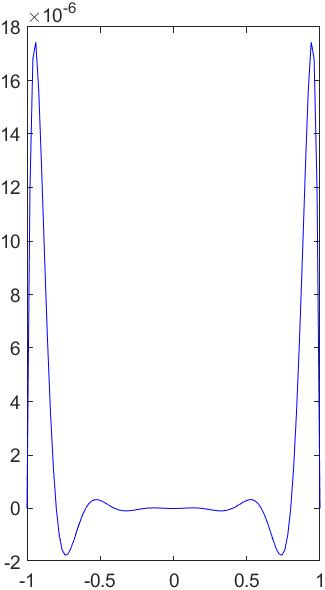
\includegraphics[width=150pt]{1.jpg}}
	\caption{[-1,-1]}
\end{figure}
\newpage
The second figure is the curve on $[-2,2]$.
\begin{figure}[h]
	\centering{
		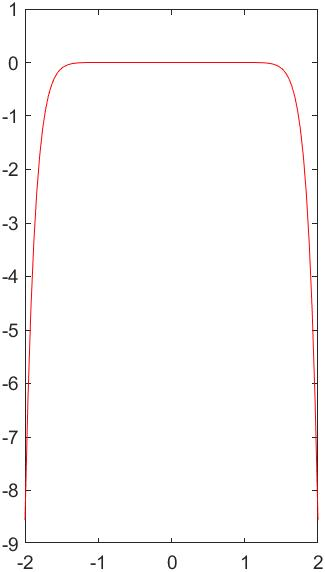
\includegraphics[width=150pt]{2.jpg}}
	\caption{[-2,2]}
\end{figure}
\end{itemize}
\end{homeworkProblem}

\end{CJK*}
\end{document}
